% ----- formatovani dokumentu -----------------------------------------------
\documentclass[12pt,a4paper,titlepage,final]{report}
\usepackage[utf8]{inputenc}
\usepackage[T1, IL2]{fontenc}
\usepackage{graphicx}
\usepackage{epstopdf}
\usepackage[margin=2cm]{caption}
\usepackage[top=3cm, left=2cm, right=2cm, text={17cm, 24cm}, ignorefoot]{geometry}
\usepackage{color}

% ------ commands -----------------------


% ---------------------------------------

\usepackage{url}
\usepackage{setspace}
\singlespacing
\usepackage[square, numbers]{natbib} 
\pagestyle{plain}
\pagenumbering{arabic}
\setcounter{page}{1}

\setlength{\parindent}{1cm}	
\usepackage{natbib}
\renewcommand{\thesection}{\hspace*{-1.0em}}
\renewcommand{\thesubsection}{\arabic{subsection}}



% ----- vyberte jazyk -------------------------------------------------------
\usepackage[english,czech]{babel}
%\usepackage[english]{babel}

% ----- dopiste titulky -----------------------------------------------------
\newcommand\Course{Zpracování obrazu}
\newcommand\WorkTitle{Detekce hran s využitím dynamického programování}
\newcommand\AuthorA{Pavel Macenauer}
\newcommand\AuthorB{Jan Bureš}
\newcommand\AuthorAEmail{xmacen02@stud.fit.vutbr.cz}
\newcommand\AuthorBEmail{xbures19@stud.fit.vutbr.cz}
\newcommand\Faculty{Fakulta Informačních Technologií}
\newcommand\School{Vysoké Učení Technické v Brně}

\usepackage[
pdftitle={\WorkTitle},
pdfauthor={\AuthorA\AuthorB},
bookmarks=true,
colorlinks=true,
breaklinks=true,
urlcolor=blue,
citecolor=blue,
linkcolor=blue,
unicode=true,
]
{hyperref}


% ----- titulni strana ------------------------------------------------------

\begin{document}
	\begin{titlepage}
	\begin{center}
		
\includegraphics[height=5cm]{images/logo.eps}
	\end{center}
	\vfill
	\begin{center}
		\begin{Large}
			\Course\\
		\end{Large}
		\bigskip
		\begin{Huge}
			\WorkTitle\\
		\end{Huge}
	\end{center}
	\vfill
	\begin{center}
		\begin{large}
			\today
		\end{large}
	\end{center}
	\vfill
	\begin{flushleft}
		\begin{large}
			\begin{tabular}{lll}
				Autor: & \AuthorA, & \url{\AuthorAEmail} \\
				& \AuthorB, & \url{\AuthorBEmail} \\
		
				& & \\
				& \Faculty \\
				& \School \\
			\end{tabular}
		\end{large}
	\end{flushleft}
\end{titlepage}		

	
% ----- obsah --------------------------------------------------------------
	
\tableofcontents

% ----- obsah -------------------------------------------------------------
\newpage
\section{Dynamické programování a detekce hran}

Dynamické programování \textbf{(DP)} stojí na Bellmanovo principu optimality, který zjednodušeně říká, že: zbývající část optimální strategie je rovněž optimální, pokud proces začíná ve stavu, do kterého se dostal v důsledku použití optimální strategie.

Na detekci hran pomocí DP můžeme nahlížet i jako na grafový problém, kdy hledáme cesty grafem, které reprezentují hrany.

\begin{figure}[ht]
\begin{center}
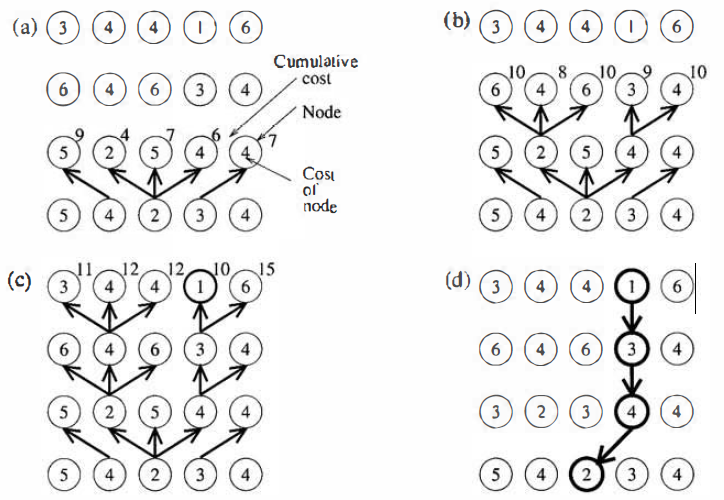
\includegraphics[width=12cm]{images/theory.png}
\caption{Princip DP při detekování hran}
\label{fig:theory}
\end{center}
\end{figure}

Minimální cesta grafem pak reprezentuje potenciální hranu. Při výpočtu ohodnocení se postupuje v DP po úrovních - pro zjednodušení např. po sloupcích, ale může se jednat i o řádky nebo jinou formu.

\begin{enumerate}
	\item Vypočtou se ceny uzlů v prvním sloupci
	\item Prochází se obraz po sloupcích, kdy se vypočte cena uzlu a zjistí minimální předek. Předek se vybírá ze sousedních pixelů v předchozím sloupci. Rozdíl Y souřadnice nemusí být pouze v intervalu $<-1;1>$. Cena předka se pak přičte k akumulované ceně uzlu.
	\item Ve chvíli kdy dojdeme na poslední úroveň. Sledujeme minimální cestu zpět. Je proto vhodné si pro výpočet uchovávat tabulku indexů pixelů ukazující na své předky.
\end{enumerate}

\paragraph{Převod na polární souřadnice} Problém u lineárního průchodu obrazem je ten, že kulaté objekty lze detekovat jen těžce. I přes sebelepší cenovou funkci se nejspíše průchod pouze "sveze" po hraně a bude pokračovat stále dál. Při lineárním průchodem polárního prostoru se kulaté objekty začnou tvářit jako lineární a s tím už DP problém nemá. Následně stačí pouze přepočítat detekované souřadnice zpět.

\begin{figure}[ht]
\centering{
	\begin{tabular}{ll}
			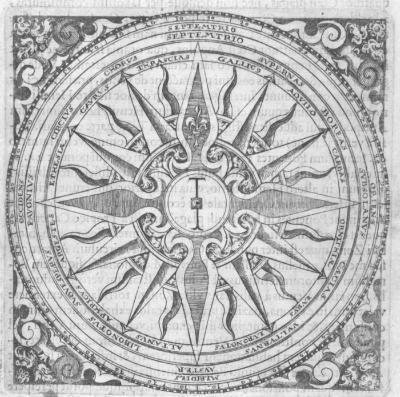
\includegraphics[height=60mm]{images/polar2.jpg} &		
			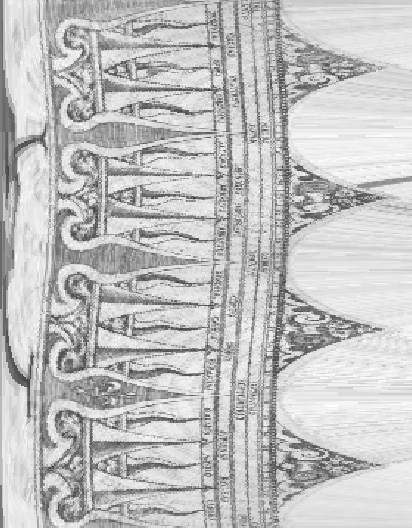
\includegraphics[height=60mm]{images/polar.jpg}
		\end{tabular}}
		\caption{Kulatý obraz v polárních souřadnicích}
\label{fig:snimac}
\end{figure}

\section{Cenové funkce}

Při detekci hran je důležité vytvořit cenovou funkci, kterou je ohodnocen každý pixel a přechod mezi jednotlivými pixely (viz. Obrázek 3). Můžeme tedy mít dvě funkce. Jednu (na obrázku 1 jako funkce h), která přiřazuje hodnotu pixelu podle jeho vlastností a druhou (na obrázku 1 jako funkce f), která urči cenu přechodu mezi dvěma pixely.  Výslednou hodnotu (na obrázku 3 jako funkce g) získáme součtem výsledků těchto dvou funkcí. Pokud se do požadovaného pixelu můžeme dostat z více předchozích pixelů je jako předchůdce zvolen ten s nejmenší hodnotou výsledné cenové funkce g. 

\begin{figure}[ht]
\begin{center}
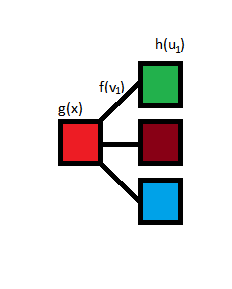
\includegraphics[width=6cm]{images/cenovefce.png}
\caption{Cenové funkce}
\label{fig:theory}
\end{center}
\end{figure}

V naší aplikace jsou využity tyto 4 způsoby určení ceny přechodů mezi pixely:

\paragraph{Rozdíl RGB složek pixelů}
Tato cenová funkce je vypočtena na základě rozdílnosti jednotlivých barevných složek dvou pixelů. Cenová hodnota samostatného pixelu je tvořena součtem cen všech předchozích přechodů, které vedly do daného pixelu. Hodnota počátečního pixelu detekce hrany je 0.

\paragraph{Rozdíl CMYK složek pixelů}
Každý pixel je nejprve převeden do barevného modelu CMYK. Následné je spočítán rozdíl každé barevné složky. Hodnota přechodu je pak tvořena součtem všech rozdílů barevných složek. Stejně jako u předchozí funkce je cenová hodnota pixelu tvořena součtem cen všech předchozích přechodů, které vedly do daného pixelu. Hodnota počátečního pixelu je taktéž 0.

\paragraph{Převod odstínů šedé}
Hodnota přechodu je spočítána tak, že se nejprve vypočte hodnota šedé barvy, kterou by měl daný pixel při převodu na odstíny šedé a spočítá se rozdíl těchto hodnot mezi dvěma pixely. Hodnotu pixelů tvoří součet všech předchozích cen hran, které vedly do tohoto pixelu. Hodnota počátečního pixelu je stejně jako u předchozích dvou funkcí nulová.

\paragraph{Intenzita a gradient}
$$ E_{sum} = C_{discont}E_{discont}(p_{i-1},p_{i})-C_{int}E_{int}(p_{i})-C_{grad}E_{grad}(p_{i}) $$

Cena uzlu je vypočítána pomocí předchozího vzorce, kde $C$ určuje váhu dané složky a $E$ energii, resp. ohodnocení. Pomocí vah můžeme experimentovat s jednotlivými složkami. $Discont$ pak určuje sousednost/diskontinuitu předchozího pixelu a jeho cenu. Předchozí pixely nemusí být jen ve vzdálenosti 1, ale můžeme zvažovat i pixely ve vzdálenosti 2 nebo vyšší.

$Int$ značí intenzitu pixelu, kdy čím vyšší intenzita, tím světlejší pixel. Je to tak vhodné pokud prohledáváme např. rentgenové snímky na černém pozadí.

$Grad$ značí gradient nebo-li přechod. Maximální hodnoty na nabývá ve chvíli, kdy je rozdíl intenzit sousedních pixelů maximální.

\begin{figure}[ht]
\begin{center}
		\begin{tabular}{lll}
			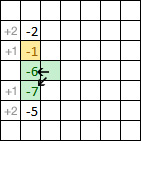
\includegraphics[height=50mm]{images/disc.jpg} &		
			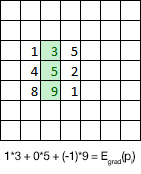
\includegraphics[height=50mm]{images/grad.jpg} &
			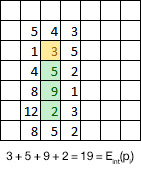
\includegraphics[height=50mm]{images/int.jpg}
		\end{tabular}
		\caption{Výpočet diskontinuity, gradientu a intenzity}
		\label{fig:theory}
\end{center}
\end{figure}

\section{Výsledky}

\paragraph{Lineární detekce hran}
Lineární detekce hran - neboli procházení zleva-doprava, odshora-dolu. Dle výsledků je vidět, že při průchodu obrazem se cesta chytá na příslušné hrany, nicméně problémy a především nápady na jejich řešení jsou následující.


\begin{itemize}
	\item Detekovat cesty v různých částech obrazu. Detekce začíná vždy z jedné strany. Ve chvíli, kdy je pozadí jednobarevné, tak jde spíše o náhodu, že cesta natrefí na nějakou hranu poté, co projde segmentem obrazu, který je jednobarevný s minimálním rozdílem intenzity. Toho by mohlo jít docílit např. vyhledáním značných rozdílů cen mezi sousedními pixely, neb tak by se velmi pravděpodobně jednalo o část nějaké hrany a z těchto bodů by pak na základě principu optimality šlo začínat.
	\item Více průchodů - složení vertikálního a horizontálního průchodu zaručí více hran.
\end{itemize}


\begin{center}
\begin{tabular}{ll}
			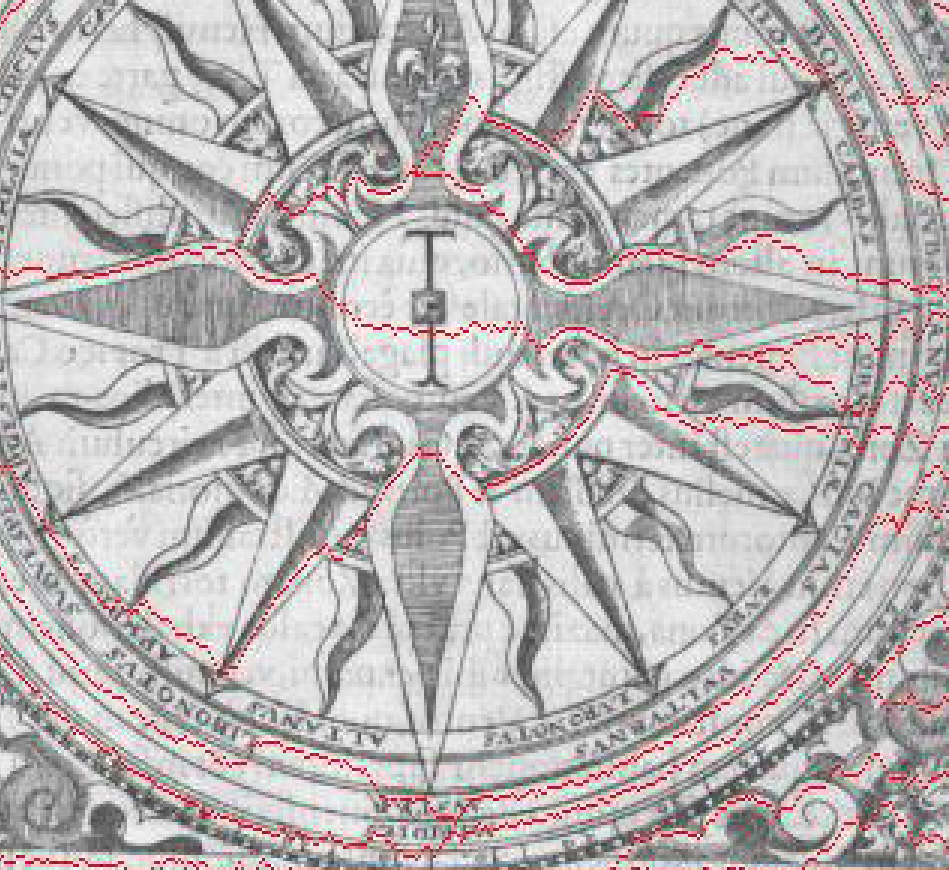
\includegraphics[height=65mm]{images/300p-res.jpg} &		
			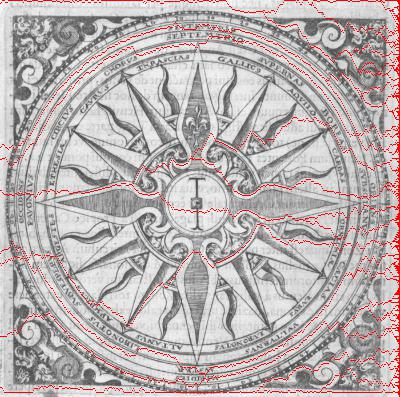
\includegraphics[height=65mm]{images/res-left-right.jpg} 
		\end{tabular}	
	
	\vspace{3mm}


\begin{tabular}{ll}
			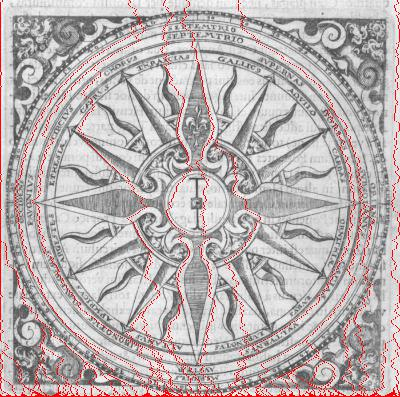
\includegraphics[height=60mm]{images/res-top-bottom.jpg} &
\centering{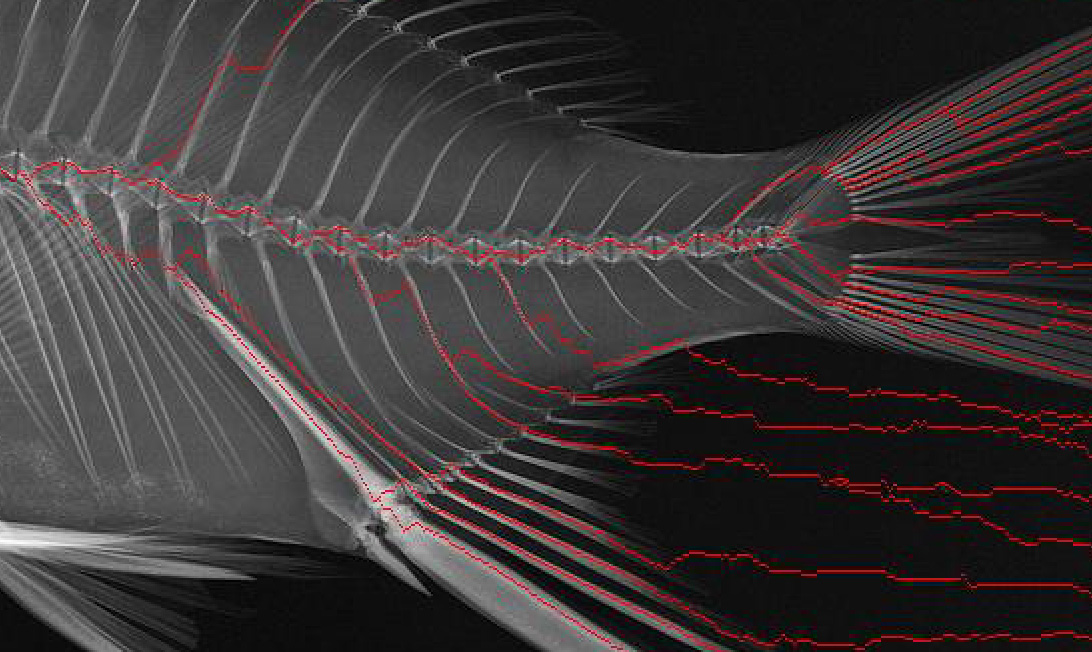
\includegraphics[height=60mm]{images/fish.jpg}}
		
		\end{tabular}	
\end{center}

					

\paragraph{Polární detekce hran}

Dalším problémem, který vyvstal je, že pomocí lineárního průchodu není možné detekovat hranu kolem kulatých objektů. Napadlo nás tak, že převodem na polární souřadnice lze kulaté objekty "narovnat", detekovat tak jejich hranu lineárně a přepočítat souřadnice zpět na kartézské.

Problémy tohoto převodu jsou především, polární souřadnice jsou dány vektorem a úhlem, který svírá s počátkem souřadné osy. Při iterování pak v zásadě kroužíme dokola a zvyšujeme poloměr. Rozlišení pro detekování hrany tak není ve všech částech obrazu stejné. Zhoršuje se v rozích polárního prostoru.

Zajímavým poznatkem také je, že pomocí této metody lze obraz segmentovat. Ve chvíli kdy se vhodně určí střed polárního prostoru je detekce hran velmi efektivní a od daného středu rozdělí obraz do více částí.
\begin{figure}[ht]
\begin{center}
		\begin{tabular}{ll}
			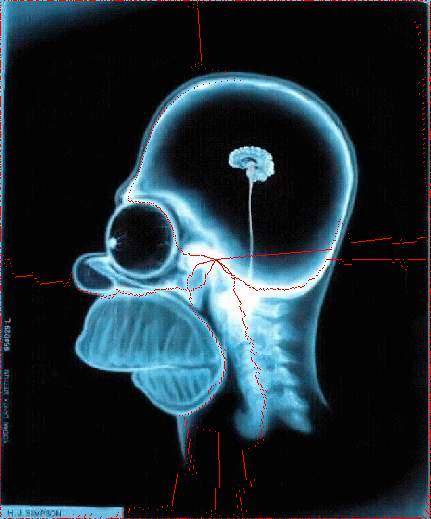
\includegraphics[height=90mm]{images/homer-polar.jpg} &		
			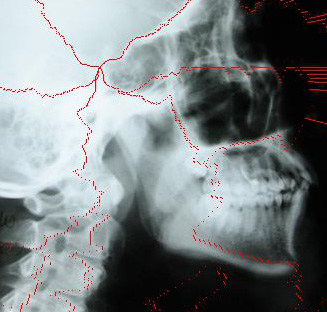
\includegraphics[height=90mm]{images/skull.jpg}
		\end{tabular}
		\end{center}
\end{figure}

\section{Obsluha programu}

Jedná se o jednoduchou GUI aplikaci spustitelnou pomocí \verb|dynamic-edge-detection.exe| na Windows. V záložce soubor načteme obrázek, který se zobrazí v levé části GUI. V prostřední části pak zvolíme typ cenové funkce (více v sekci Cenové funkce). Směr průchodu grafem. Je možné nastavit průchod zleva-doprava, shora-dolů nebo pomocí polárních souřadnic. Jemnost pak určuje jemnost vykreslení. Následně už jen nastavíme barvu hrany a klikneme na tlačítko Detekuj hrany. Výsledek se zobrazí v pravé části aplikace.

\paragraph{Kompilace} Aplikace je multiplatformní. Ve složce \verb|src| je přiložen projekt v Qt Creatoru využívajícího qmake. Stačí tedy použít standardní Qt nástroje ke kompilaci pro Linux a další platformy podporující knihovny Qt.

\paragraph{Referenční obrázky} Ve složce \verb|test-images| jsou obrázky používané pro testování

\bibliographystyle{plain}

\nocite{cite1}
\nocite{cite2}
\nocite{cite3}
\nocite{cite4}
\nocite{cite5}

\hypertarget{bib}{}
\bibliography{reference}
\addcontentsline{toc}{section}{Literatura}

\end{document}

